\section{Design and Requirements}
\label{sec:design}

The Marketplace provides a database of available appliances, allowing
users to find appliances of interest and administrators to validate
those appliances.  To make the database easily accessible it is
implemented as a web service permitting both programmatic and
browser-based access.  The design and implementation are agnostic with
respect to the cloud distribution, allowing any cloud distribution to
interface to the Marketplace\@.

Table~\ref{tab:requirements} contains a detailed list of requirements
for the Marketplace as an appliance registry and for the appliance
metadata.\footnote{References prefixed with `RU' or `RS' in the
  following text refer to the requirements in this table.}  The core
requirements have been derived from the primary use cases and feedback
from the StratusLab users and administrators.

\subsection{Timeline}

A core concept within the Marketplace is the appliance timeline, a
complete history of all endorsements related to a given appliance (see
Fig.~\ref{fig:timeline}).  An appliance can be endorsed by more than
one person to allow for third party validation and approval of
appliances. [RU3] Moreover, a particular endorser may change her
endorsement over time, updating the metadata data associated with the
appliance or explicitly deprecating the appliance. [RU2] Endorsements
are also time-limited, containing an explicit validity period.

Users of the Marketplace can retrieve the full history, for example to
conduct an audit on why a particular appliance was authorized at a
particular point in time.  Normally however, the Marketplace users
only want to see the current endorsements for an appliance, that is
the list of the latest, non-expired endorsements from all of the
endorsers of an appliance.  This allows users and administrators alike
to decide if an appliance is currently valid.

\begin{figure}
\begin{center}
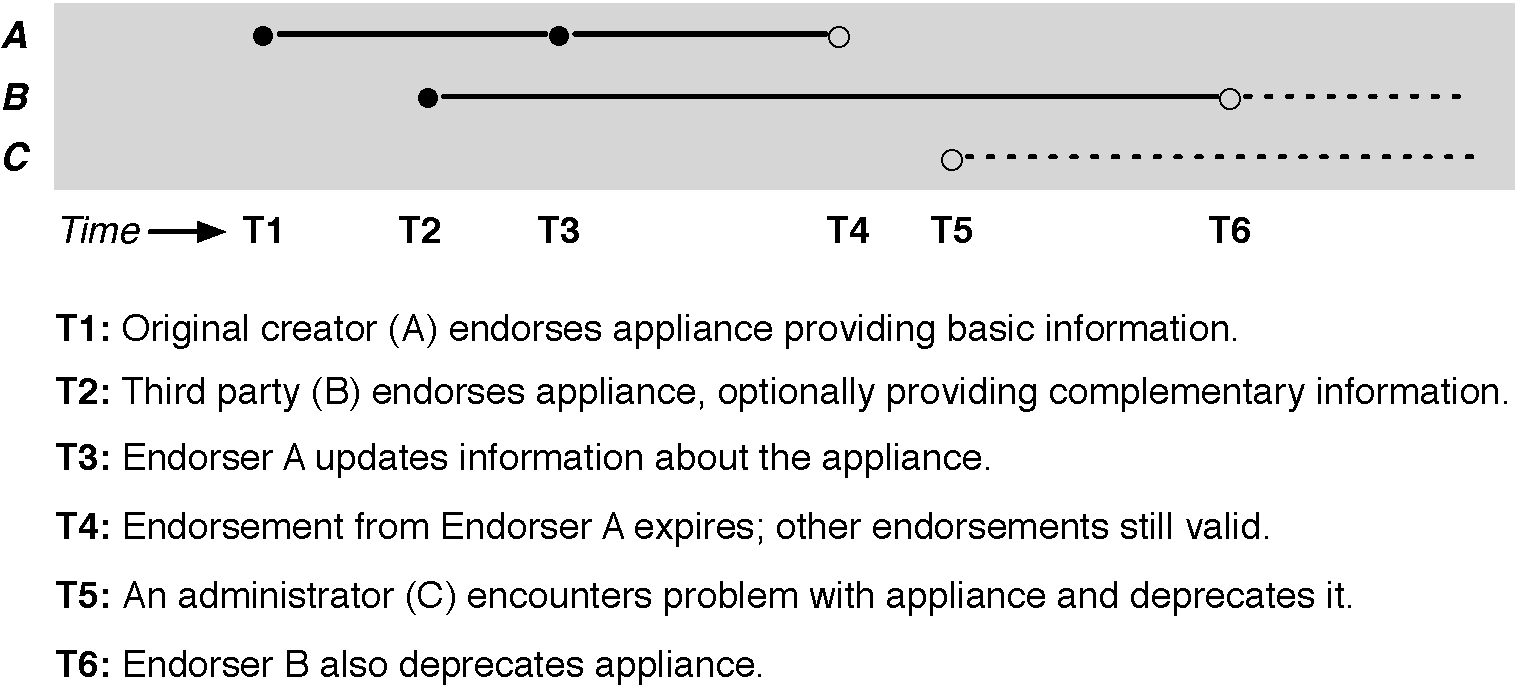
\includegraphics[width=\columnwidth]{timeline.pdf}
\end{center}
\caption{Timeline for an appliance.  The dots represent the metadata
  entries created by endorsers A, B, and C\@.}
\label{fig:timeline}
\end{figure}

\subsection{Separation of Metadata and Appliance Contents}

A conscious design decision was made to separate the storage and
transport of appliance contents from the Marketplace implementation.
Storing the appliance contents outside of the Marketplace makes it
easier to:
\begin{itemize}
\item Scale the Marketplace implementation,
\item Create mirrors of the Marketplace,
\item Ensure the implementation is independent of the transport
  protocol
\item Allow owners of the image to control access to the appliance
  contents, and
\item Relieve the Marketplace operator of the Marketplace from
  copyright and licensing concerns.
\end{itemize}
It also allows the StratusLab distribution to take advantage of
standard web servers or other cloud storage services for the appliance
contents.

\begin{table}
\caption{Requirements}
\label{tab:requirements}
\begin{center}
\begin{tabular}{lp{0.85\columnwidth}}
\hline\hline

\\ RU1 & Anyone with a valid email address can upload metadata
descriptions to the Marketplace\@.

\\ RU2 & Users can ``replace'' existing metadata descriptions by
uploading a new signed description(s).

\\ RU3 & Multiple metadata entries may be associated with a particular
appliance, allowing third parties to endorse images.

\\ RU4 & All validated descriptions uploaded to the site must always
be available to provide a timeline of the metadata evolution.

\\ RU5 & Users must be able to search the metadata database on a
reasonable subset of the possible keys, for example the image
identifier and the endorser's email address.

\\ RU6 & The registry should allow the metadata to be downloaded in
alternate formats, notably JSON and HTML.

\\ RU7 & The service must be easy to access from all programming
languages (including scripting languages) and usable from a web
browser.

\\ RU8 & The underlying schema for the metadata entries must be
flexible and extensible, to account for different and evolving needs.

\\ RU9 & Entries should contain at least one location from which the
appliance can be obtained; entries without a location are
appropriate only for deprecated appliances.

\\

\hline

\rule{0pt}{15pt}RS1 & Metadata entries must be cryptographically
signed with the endorser information matching the information in the
certificate itself.

\\ RS2 & Metadata entries must contain a valid email address, which is
confirmed for each entry upload.

\\ RS3 & Users must be able to download the original signed metadata
in the RDF/XML format from the registry for verification.

\\ RS4 & All entries must contain a creation date for the endorsement.
The server must only accept descriptions with a creation date more
recent than the current latest.

\\ RS5 & It must be possible to unambiguously associate an entry to an
appliance and to verify the integrity of the appliance.

\\
\hline\hline
\end{tabular}
\end{center}
\end{table}
